\section{A Review of Smart Data Pricing}\label{sec:congestion}

Smart data pricing encompasses a wide variety of different pricing algorithms and proposals. In this section, we briefly discuss some of these ideas, following the taxonomy given in Figure \ref{fig:taxonomy}. We include a brief overview of related pricing plans in the electricity and transportation industries, which can help yield insights into the feasibility of various forms of SDP for data, as well as ideas for new pricing plans. Other, more thorough reviews may be found in \cite{CourcoubetisWeber,sen2013survey,Songhurst}.

\begin{figure}
\centering
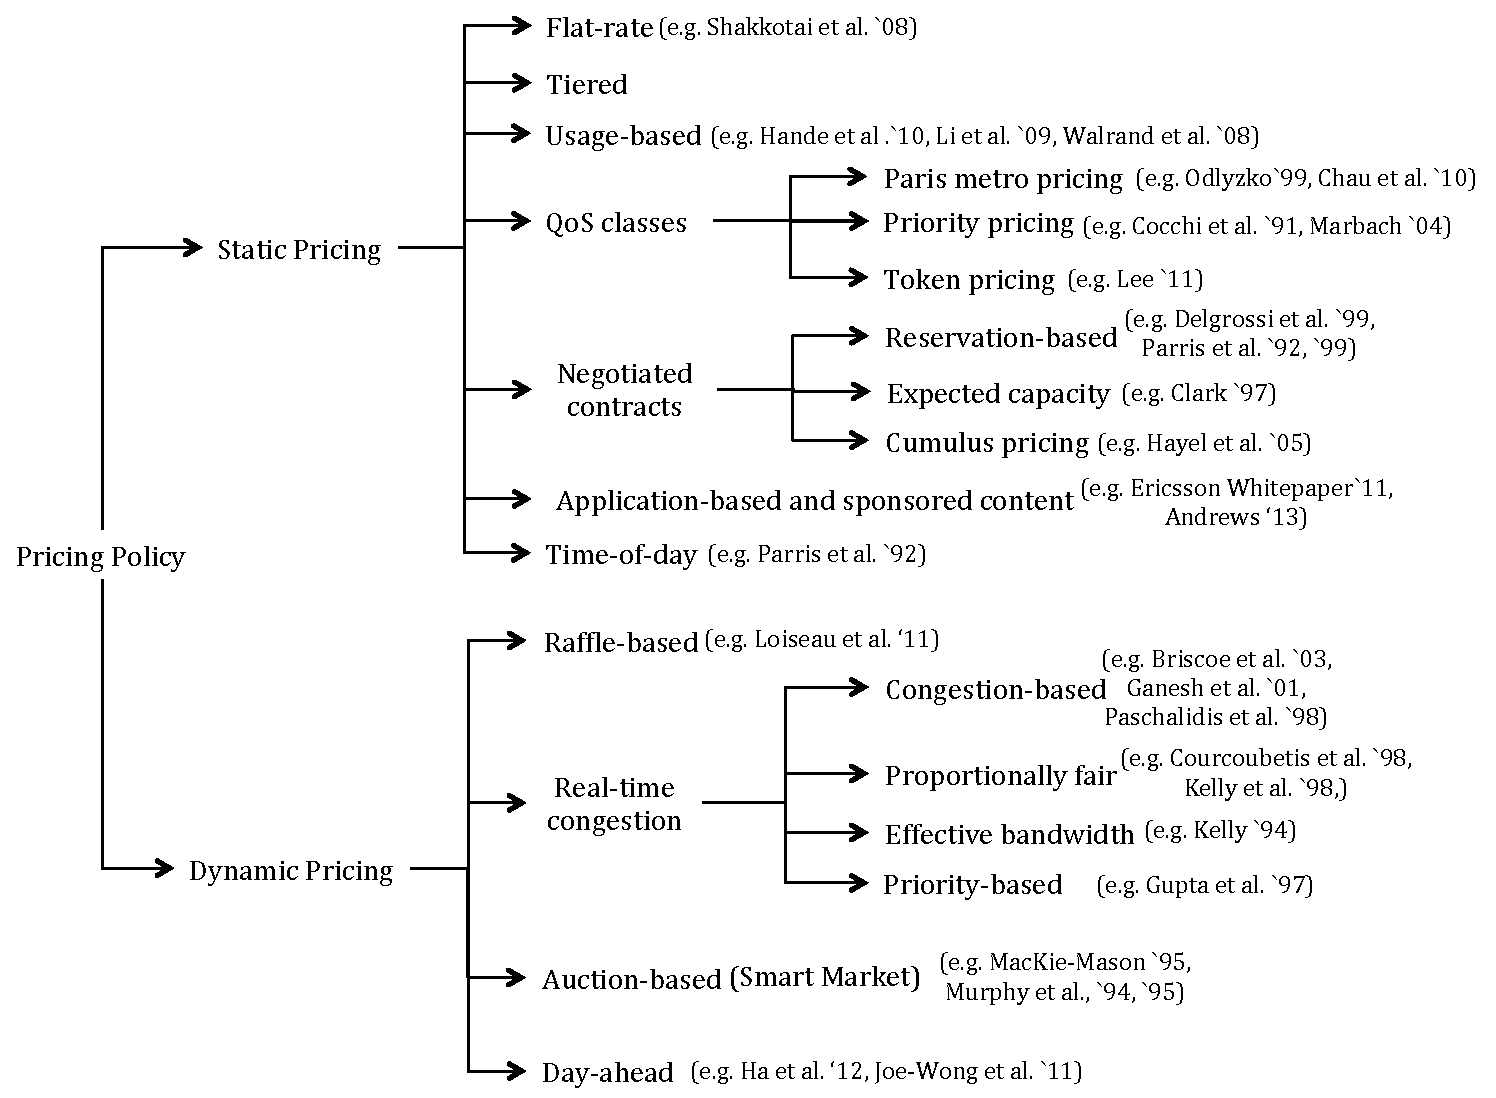
\includegraphics[width = 0.8\textwidth]{Figures/Taxonomy.pdf}
\caption{Examples of broadband pricing plans proposed in the research literature.}
\label{fig:taxonomy}
\end{figure}

A primary goal of SDP is to create the right incentives (or price points) for users to modify their usage behavior so as to help ISPs with better resource allocation and utilization. But creating these incentives requires ISPs to account for users' responses to the prices offered. Of particular relevance is the timescale associated with the pricing mechanism -- do the prices continually change as the network load changes? If so, how frequently and by how much? How to balance the trade-offs between users' reluctance to real time dynamic pricing and the inability of static pricing to exploit the time elasticity of demand of different applications in congested times? How to balance the trade-offs between the users' need for transparency and control over her usage and the need for automation in dynamic pricing scenarios? 

\emph{Static pricing} plans are those that change prices on a relatively longer timescale, e.g., months or years: the offered prices do not vary with immediate changes in the network congestion level. The popularity of these plans arises from the certainty they provide to a user's expected monthly bill. For instance, tiered data plans with pre-specified rates are prevalent in the United States, and several European and Asian ISPs offer usage-based pricing in which users are charged in proportion to their usage volume. But such usage-based pricing leaves a timescale mismatch: ISP revenue is based on monthly usage, but peak-hour congestion dominates its cost structure (e.g., network provisioning costs increase with the peak-hour traffic). Another well-known pricing plan is time-of-day (ToD) pricing, in which users are charged higher prices during certain ``peak'' hours of the day. But even with ToD pricing, the hours deemed as ``peak'' are fixed, which results in two challenges. First, traffic peaks arise in different parts of the network at different times, which can be hard to predict in advance and could end up creating two peaks during the day--one during peak periods, for traffic that cannot wait for several hours for lower-price periods, and another peak during discounted ``off-peak'' periods for time-insensitive traffic. Such patterns have been observed in dynamic pricing for voice calls in operational networks \cite{Economist}. We discuss several of these existing static pricing plans and proposals in greater detail in Section \ref{sec:static}.

\emph{Dynamic pricing} takes the ToD idea further in that it does not pre-classify peak and off-peak periods, instead adjusting prices at a finer timescale or by location in response to the network congestion. However, prices that vary depending on the current network load can be sometimes inconvenient for users.  Hence, dynamic pricing variants for SDP, such as automated ``smart market" \cite{MacKie-Mason,Murphy-Murphy}, raffle-based pricing \cite{loiseau2011incentive}, and day-ahead pricing \cite{ha2012tube}, have been proposed to guarantee the prices a day in advance to give users some certainty about the future prices on offer. Each day, new prices are computed for different times (e.g., hours) of the next day, based on predicted congestion levels.  A detailed discussion on these dynamic pricing proposals will be provided in Section \ref{sec:dynamic}.


\subsection{Static Pricing}\label{sec:static}

Due to the fixed nature of their prices, static data plans do not generally allow ISPs to adapt to real-time congestion conditions. In particular, the ISP cannot prevent or alleviate network congestion at peak times by manipulating the prices. On the other hand, static pricing tends to be more acceptable to users, as it offers more certainty and is simpler than dynamically changing prices. Indeed, the most basic form of static pricing, \emph{flat pricing}, is also the most simple for users, though it does not impose any sort of usage incentives \cite{shakkotai}. Some other important examples of static pricing include the following:

\textbf{\emph{Usage-based:}}
In its purest form, usage-based pricing charges users in proportion to the amount of data that they consume, without regard to the type of data (e.g., application) or time of consumption. The principal advantage of such a pricing plan lies in its relative simplicity: it imposes a monetary penalty on heavy (i.e., high-usage) users to reduce congestion \cite{hande,Li}, but also penalizes users even when the network is lightly loaded. Moreover, usage-based pricing requires users to keep close track of their usage in order to determine how much they have spent on data \cite{walrand}.

\textbf{\emph{Tiered:}}
A more common variant of pure usage-based pricing is tiered pricing, in which users pay a fixed amount of money for a monthly \emph{data cap} (e.g., \$30 for 3GB). This fixed fee covers usage up to the cap, after which users may pay another fixed fee to increase the cap by a discrete amount, e.g., \$10 per extra GB. Thus, tiered or capped pricing can be viewed as a discretization of usage-based pricing. Many ISPs have adopted such a pricing plan or another variant in which the data cap is shared across several devices (i.e., a \emph{shared data plan}). Like usage-based pricing, tiered pricing is simple for users to understand and penalizes heavy usage. %; however, it also puts less burden on users to keep track of their usage in order to calculate their monthly bills. % Yet neither usage-based nor tiered pricing prevents users from using the network at the same time, and thus do not significantly help reduce the peak congestion. 

\textbf{\emph{Quality of Service (QoS) classes:}}
Some static pricing plans offer multiple traffic classes with different qualities of service (QoS). A simple differentiated pricing plan is \emph{Paris metro pricing} (PMP), which is named after an actual pricing practice on the Paris metro in the 1900s \cite{Odlyzko}. In Paris metro pricing, the ISP separates data traffic into different logical traffic classes and charges different prices for logically separate traffic classes (i.e., each class is identical to the others in their treatment of data packets). Only users willing to pay a higher price will adopt this traffic class, which leads to a better QoS due to fewer users. But one of the key issue of academic debate related to PMP has been its viability, namely,  whether it is a mechanism to increase the profits for service providers, or whether it achieves higher social welfare. As pointed out in \cite{Chiu2010}, the conclusions of this debate depend on how users react to the congestion externality of the underlying system. Other researchers have investigated more direct forms of QoS pricing, in which users can indicate their desired QoS in their packets and are charged a higher per-byte fee for higher QoS \cite{Cocchi1,Marbach,M3I}. %Determining users' optimal QoS decisions and the per-byte fees to charge are non-trivial research questions.

%each of which is identical in its treatment of data packets but charges users differently.  Thus, users willing to pay more will select the more expensive, and hence less congested, logical traffic class.

Another form of QoS pricing is \emph{token pricing}, in which users receive tokens at a fixed rate (e.g., 1 per minute) \cite{Token}. Users can then spend these tokens to send some of their traffic at a premium QoS; users can choose the timing of these premium sessions, e.g., to coincide with their individual priorities and preferences. %One can then examine users' spending decisions and their implications for congestion reduction.

\textbf{\emph{Negotiated contracts:}}
In these types of pricing schemes, users pre-negotiate contracts with the ISP regarding the price of sending traffic over the network. The main research question for such contracts is then characterizing this user-ISP interaction and both parties' optimal decisions. For instance, in \emph{reservation-based pricing}, users specify a monthly budget for data; the ISP can then accept or reject users' connections based on users' remaining budget and the real-time network congestion \cite{Delgrossi,PKF, ParrisF}. 

In \emph{expected capacity pricing}, Clark proposed a mechanism in which users similarly negotiate a price in advance based on an ``expected'' quality of service (e.g., file transfer time), so that at congested times the ISP can freely allocate network resources based on whether a given packet lies ``within'' a user's purchased traffic profile \cite{DDClark}. The goal of this pricing scheme is to ``\emph{provide additional explicit mechanisms to allow users to specify different service needs, with the presumption that they will be differentially priced} \cite{DDClark}." Expected capacity pricing allows users to explicitly specify their service expectation (e.g., file transfer time), while accounting for differences in applications' data volume and delay tolerance. The idea is that by entering into profile contracts for expected capacity with the operator, different users should receive different shares of network resources when the network gets congested \cite{Songhurst}.  
One specific proposal to realize this service involved traffic flagging (i.e., each packet is marked as being \emph{in} or \emph{out} of the user's purchased profile, irrespective of network congestion level) by a traffic meter at access points where the user's traffic enters the network. This is followed by congestion management at the switches and routers where packets marked as \emph{out} are preferentially dropped during congested periods, but are treated in an equal best-effort manner at all other times.  The expected capacity is thus not a capacity guarantee from the network to the user, but rather a notion of the capacity that a user expects to be available and a set of mechanisms that allow the user to obtain a different share of the resource at congested times.  
%This pricing can be simply enforced at the router and switches of the network, and allows service providers to have more stable estimates of the future necessary capacity based on the total expected capacity sold, rather than the sum of peak rates of all users' access links.  A dynamic pricing version of the scheme has also been explored \cite{DDClark}. However, in order to implement this pricing scheme, the assignment of price values to expected capacity profiles requires further study.

An ISP offers similar contracts under \emph{cumulus pricing}, but users can re-negotiate the price after passing ``cumulus'' usage points \cite{Hayel}. Cumulus pricing consist of three stages: specification, monitoring, and negotiation. A service provider initially offers a flat-rate contract to the user for a specified period based on the user's estimate of resource requirements. During this time the provider monitors the user's actual usage and provides periodic feedback to the user (by reporting on ``cumulus points'' accumulated from their usage) to indicate whether the user has exceeded the specified resource requirements. Once the cumulative score of a user exceeds a predefined threshold, the contract is renegotiated. 

\textbf{\emph{App-based and sponsored content:}}
Different applications consume different amounts of data traffic (e.g., streaming video consumes much more data than retrieving emails). Some researchers have thus proposed app-based pricing, in which users are charged different rates for different apps \cite{Ericsson}. Such pricing plans also include ``zero-rated'' apps, whose traffic is free for the user. A variant of such pricing schemes is ``sponsored content'', in which a third-party (advertiser, content provider, or the ISP itself) ``sponsors'' some part of the traffic in return for accessing specific content or using data at less congested times. 

App-based plans have been offered in Europe, largely on a promotional basis. However, app-based pricing presents technical challenges for ISPs-- ISPs need to identify and track how much data each user consumes on specific applications, which may raise privacy concerns. Moreover, some apps open links in separate apps (e.g., links in Flipboard may open a separate Internet browser), creating confusion among users as to the app to which some traffic belongs, and whether this traffic counts towards the sponsored volume or not. Even in academia, sponsored content research is relatively sparse, though a few initial models have been developed \cite{andrewsSDP,hande2009network}.

\textbf{\emph{Time-of-day (ToD):}} ToD pricing charges users different usage-based rates at different times of the day (e.g., peak and off-peak hours) \cite{ParrisF}. The free nighttime minutes offered for voice calls by most US ISPs before 2013 are one simple form of ToD pricing. However, as the peak times and rates are fixed in advance, ToD pricing can end up creating two peaks, one during the ``peak'' period and one in the ``off-peak'' period; indeed, this phenomenon was observed in Africa when MTN Uganda offered discounted prices for voice calls made at night. 

Some ISPs offer two-period ToD pricing plans with different charging rates at day and night times.  For example, BSNL in India offers unlimited night time (2-8 am) downloads on monthly data plans of Rs 500 (\$10) and above. Other variations of ToD pricing are offered elsewhere; for instance, the European operator Orange has a ``Dolphin Plan''  for $\pounds$15 (\$23.50 USD) per month that allows unlimited web access during a ``happy hour'' corresponding to users' morning commute (8-9 am), lunch break (12-1 pm), late afternoon break (4-5 pm), or late night (10-11 pm). The underlying idea is to allow consumers to \emph{self-select} themselves into ``time-buckets" with QoE guarantees, with the hope of exploiting the variance in consumers' time-of-day preference to spread out demand more evenly over the day.


%Though the prices do change with time in ToD pricing, we list ToD pricing under static pricing due to the fact that the prices remain the same from day to day.

\subsection{Dynamic Pricing}\label{sec:dynamic}
Dynamic pricing allows prices to be changed in (near) real-time, which unlike static pricing allows an ISP to adjust its prices in response to observed network congestion. However, in doing so the ISP significantly complicates its pricing, making it much harder for users to understand. Thus, implementing and offering dynamic pricing plans requires ISPs to account for human factors that can make real-time changes in price more amenable to users. Some of the proposed dynamic pricing plans are discussed below:

\textbf{\emph{Real-time congestion:}} If ISPs can monitor their network for real-time signs of congestion, they can increase prices when congestion is observed, and decrease them when the traffic load is relatively light. Thus, there is a \emph{feedback loop} between ISPs offering prices and users correspondingly adjusting their usage \cite{Ganesh,Paschalidis}. This \emph{responsive pricing} sets prices so as to keep user demand under a certain level; if an ISP further chooses the prices so as to optimize a proportional fairness criterion on the amount of bandwidth allocated to different users, we obtain \emph{proportional fairness pricing} \cite{Courcoubetis,kelly1998rate,gibbens-kelly}. Many variants of responsive pricing have been proposed in the literature, principally as a congestion control mechanism; in practice, it would be impractical for users to manually respond to the prices offered for each Internet connection. Hence, automation of client devices (or agents) to intelligently adapt their data consumption will be necessary to realize such real-time pricing. But recent HCI studies \cite{chetty2010s,sigchi} have revealed complex patterns of household politics and user opinion regarding such decision-making about bandwidth consumption. In particular, there is a reluctance among users to delegate such bidding or scheduling to automated agents that stems from a conflict between the psychological assurance of manual control and the convenience of automation, which in turn depends on the perceived trust-worthiness of the underlying system. Many of the findings reported later in this chapter on user behavior and user interface design may serve as guidelines in designing user-friendly client-side agents to enable such pricing plans. 

Another form of congestion pricing, \emph{effective bandwidth pricing}, incorporates a form of QoS by charging users based on their connection's peak and mean rates \cite{Kelly-eff}. One can also explicitly incorporate different QoS by using \emph{priority pricing}, in which users can pay less by accepting a longer delay at congested times \cite{Gupta}. If the prices are chosen correctly, the system reaches an equilibrium, in which each user's packets are processed within the delay paid for.

\textbf{\emph{Auction-based:}} One disadvantage of real-time congestion pricing is that in practice, the ISP must set the prices (just) before observing user behavior. Since user demand can change with time, the ISP may end up setting non-optimal prices due to outdated assumptions of user demand. ``Smart market'' pricing addresses this slight delay with an auction-like scheme, in which users attach a bid to their packets that signifies their willingness to pay \cite{MacKie-Mason,Murphy-Murphy}. ISPs then admit a limited number of packets in descending order of the bids so as to limit network congestion. Users are charged the lowest bid admitted, which represents the ``cost of congestion.'' While smart market pricing allows true real-time pricing, it also requires automated agents on user devices to make bids as necessary and keep track of the final amount charged.

\textbf{\emph{Raffle-based:}} This is a variation of dynamic time-dependent pricing inspired by lottery reward mechanism. Under \emph{raffle-based pricing}, the exact price that users pay is determined after-the-fact, i.e., in a probabilistic manner that depends on the amount of data consumed by a user \cite{loiseau2011incentive}. Users have a chance to receive a monetary reward during congested times if they agree to shift their demand to less-congested times. They are entered into a lottery for a fixed reward, where the probability of winning the lottery depends on the user's contribution to the total amount of traffic shifted. While such a pricing plan is attractive to ISPs in that the total reward offered is fixed, users may be less willing to shift their traffic because of the uncertainty in winning the lottery and the reward amount, which depend on external factors like the behavior of other users.

\begin{figure}
\centering
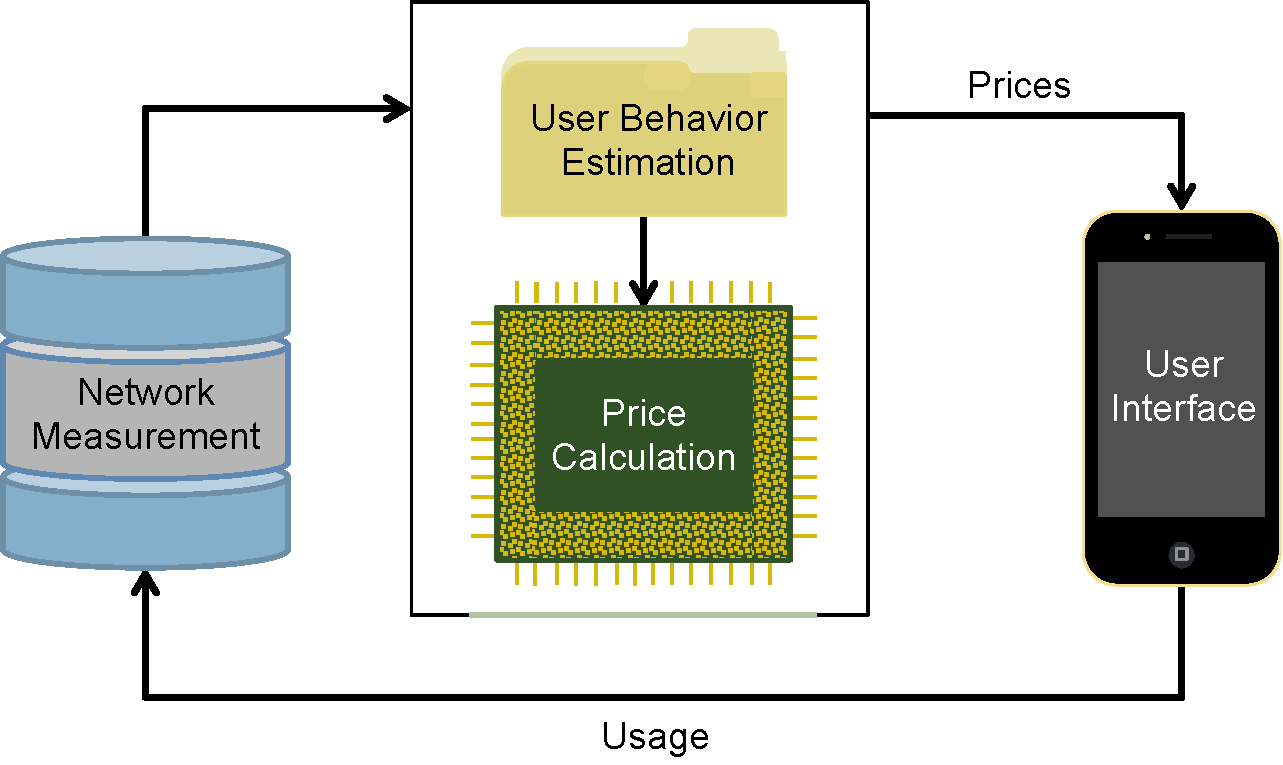
\includegraphics[width = 0.6\textwidth]{Figures/Loop_TUBE.pdf}
\vspace{-0.1in}
\caption{Feedback loop schematic of day-ahead pricing.}
\label{fig:tube-loop}
% \vspace{-0.05in}
\end{figure}

\textbf{\emph{Day-ahead time-dependent:}} In an effort to increase user certainty of the prices, ISPs can guarantee their time-dependent prices one day in advance, and continue to compute new prices to maintain this sliding one-day window of known prices \cite{ha2012tube,Carlee}. Users can then plan their usage in advance, while ISPs can adapt their estimates of user behavior and usage volume in calculating the prices for subsequent days. Day-ahead pricing thus strikes a balance between user convenience and ISP adaptability. This has been a successful pricing mechanism in the electricity market, and hence can be adapted to broadband networks with careful consideration. A schematic of the resulting feedback loop is shown in Figure \ref{fig:tube-loop}. In the next section, we examine a prototype of day-ahead pricing for mobile data in order to illustrate the ``end-to-end'' nature of an SDP deployment.

We pause to briefly compare day-ahead TDP with the other types of dynamic pricing discussed above. Real-time pricing and Smart Market mechanisms require users to delegate some control and operate in an automated mode as the time-scale is too short for user-mediated choices. On the other hand, simple 2-period (day \& night) time-of-day pricing has time scale that is too long to take advantage of any spare capacity availability and time elasticity of demand which vary at much shorter time-scale. Auction-based mechanisms will require modifications to the network equipments (e.g., agents to recognize bid amounts and perform admission control) and client side agents for automated bidding. Raffle-based pricing creates uncertainty in rewards and unless the time-varying prices are known in advance, users may be reluctant to adopt such data plans. A day-ahead dynamic time-dependent pricing plans solves many of these issues by providing guarantees on the future prices in advance, takes advantage of demand elasticities at shorter time-scales, and provides ISPs with a mechanism to optimize the prices they offer.  

But what are the challenges of realizing dynamic day-ahead time-dependent pricing?
\begin{itemize}
\item How to develop an economic model for dynamic day-ahead TDP which computes optimized prices that accounts for users' time elasticity of demand in maximizing the total revenue of the network provider? The price computation needs to consider (a) the cost incurred in offering price discounts, (b) savings from shifting some traffic from peak to off-peak hours, (c) the increase in baseline demand in discounted periods due to potential ``sales day" effect.
\item How to engineer a system that enables this pricing by developing both provider and client-side modules (in particular, the user interfaces needed for users to react to the offered prices)?
\item How can researchers carry out field trials of such pricing plans by interposing themselves as a ``bandwidth reseller" between the network providers and its real consumers?
We will address these questions in Sections \ref{sec:dayahead}, \ref{sec:psychology}, \ref{sec:engg}, and \ref{sec:TDP}.  
\end{itemize}

\subsection{Comparison with other Markets: Similarities and Differences }

Let us now take a look at what forms of time-dependent pricing have been already field tested and exist in the real world in networks that suffer from congestion problems to identify differences and opportunities for innovating TDP plans for broadband networks.   
Much like today's data networks, the electricity and transportation markets have both experienced a capacity shortage over the past decade and have developed new pricing plans to cope with the resulting shortfall. By comparing electricity usage and road traffic to data traffic, we see that these industries are quite similar to data networks, and that their pricing plans may inform SDP for mobile data. Indeed, both industries observe a highly variable demand throughout the day, allowing for both static and dynamic pricing plans.
%Over the past decade, the electricity market has experienced a capacity shortage much like that anticipated for wireless ISPs in the near future.  
In particular, time-of-day road tolls have been offered in many transportation networks, and many electricity utilities have both trial-ed and deployed time-of-day pricing. We give an overview of such pricing plans in this section, with the aim of highlighting the unique challenges posed by refining such pricing plans to accommodate broadband data networks. Figure \ref{fig:compare} gives an overview of the analogies between pricing plans proposed for the transportation, broadband, and electricity industries.

The similarities and differences between these pricing plans reflect the different industries for which they are designed. In particular, we observe the following distinctions:
\begin{enumerate}
\item
\textbf{\emph{Real-time communication:}} User devices on data networks, e.g., smartphones, are capable of real-time communication with the ISP network, for instance if the prices change in real time. But such real-time feedback for price (toll) changes in road networks is harder to realize and will require additional infrastructural support. In electricity markets, new smart grid interfaces have been developed that can display real-time prices, but individual devices, e.g., air conditioners or vacuum cleaners, generally cannot interact directly with the provider smart grid and require a smart energy controller to schedule their energy consumption.
\item
\textbf{\emph{Elasticity of demand:}} Smartphones' ability to communicate with the ISP network in real time is complemented by users' ability to easily control their usage on individual devices and applications. For instance, a user could simply stop streaming a video if the price increases; such measures could also be automated within the device. The users' decisions will reflect the large variance in the demand elasticity of different types of applications (some of which, such as software downloading, P2P, file backup may not even require user participation and can be completed in small chunks whenever low prices are available). In contrast, devices on electricity networks typically consume energy constantly as long as they are active. There is little opportunity for many devices (e.g., washer, dryer, lights) to complete their activities in an intermittent manner without requiring active user engagement. In road networks, the contrast is even more stark; users in the network (e.g., already driving) cannot easily exit or postpone their activity.
\item
\textbf{\emph{Long-term volatility:}} Most people do not have a concrete idea of how much data they consume each month, partly because most data plans charged a flat fee for unlimited access until recently. Moreover, an individual's data usage can vary greatly from day to day, as relatively casual actions such as streaming a video can have a large impact on total data consumption. In contrast, most people have a relatively good idea of how much they drive per day, and the distance traveled, and road toll fees. Thus, people may be more able to plan ahead by buying permits (e.g., EZ pass) or carpooling during congested hours. In electricity markets, household demand similarly does not vary much from day to day. Consumption of electricity is largely driven by user \emph{needs}, rather than the more volatile \emph{preferences} that drive demand for Internet data.
\end{enumerate}
% For instance, user devices on data networks, such as smartphones, are capable of real-time communication with the ISP network, and allow a user to interact with pricing policies in real time. Moreover, users are able to quickly adjust their behavior, e.g., stopping a video streaming session. With transportation networks, users cannot view real-time price adjustments or leave the network easily once they have begun driving. New smart grid technologies enable some real-time price updates, but these are not nearly as widespread as smartphones. Users can often plan ahead more readily for their transportation and electricity needs, e.g., buying permits from secondary markets at congested times. A user's data rate, however, is highly variable even on a long timescale, and most users are not aware of how much data they actually consume. Most people, however, do have an idea of how many miles they drive at what times of the day, which makes planning for road pricing particularly easy.
\begin{figure}
\centering
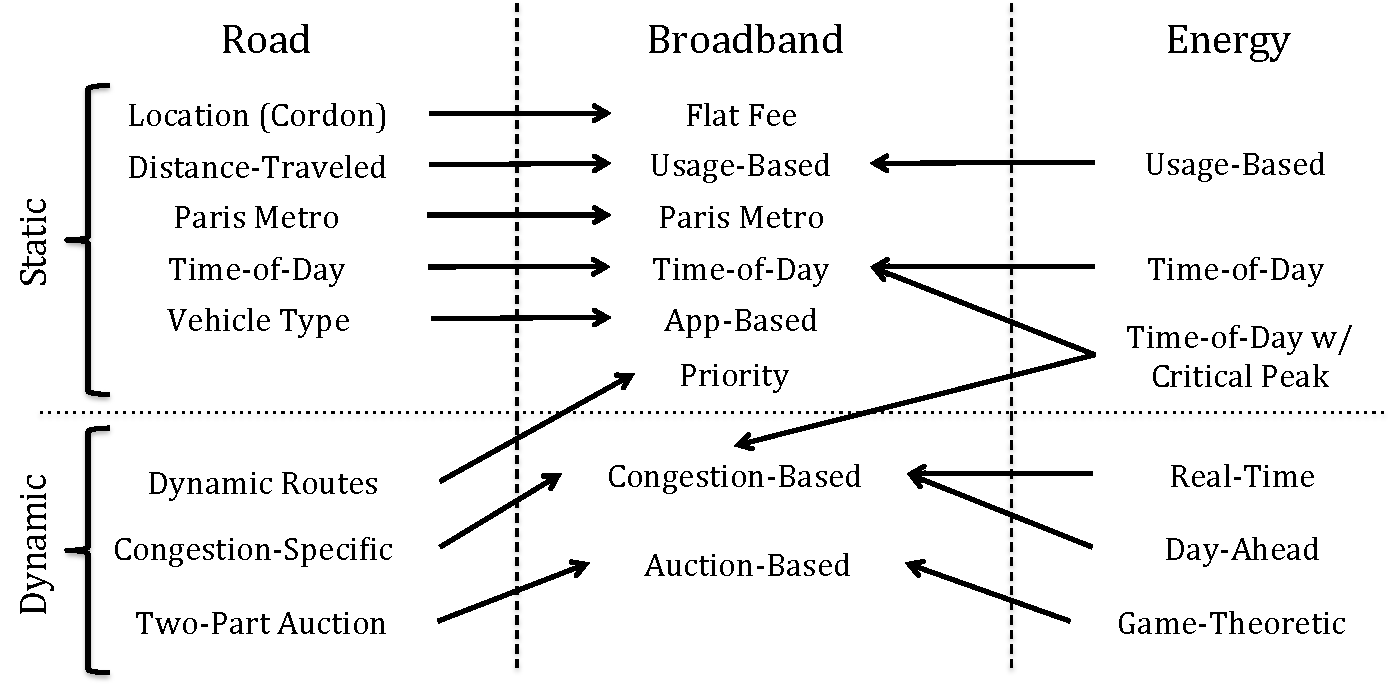
\includegraphics[width = 0.6\textwidth]{Figures/Relationships.pdf}
\caption{Comparison of pricing plans in the transportation, broadband, and electricity industries.}
\label{fig:compare}
\end{figure}
% These trials and the accompanying literature suggest that similar plans may be adopted by network operators. 
% Indeed, the electricity and broadband networks are quite similar in that data traffic can be compared to electricity usage, while different data applications are analogous to different energy-consuming household appliances.  In light of this analogy, the discussion below gives a brief overview of the existing literature on pricing for electricity industries, focusing on time-of-day and dynamic pricing.  A summary of all these pricing policies and their related literature is provided in Table \ref{references}.


\subsubsection{Static Pricing}

Traditional road pricing has been simple flat-rate cordon pricing, analogous to flat pricing of data. Pricing by vehicle type, analogous to app-based pricing for data, has also been proposed, e.g., charging trucks more than passenger vehicles \cite{ushighways}. Forms of flat-rate priority pricing have also been implemented, most obviously in the Paris metro's pricing scheme from which data networks' Paris metro pricing takes its name. High-occupancy vehicle or ``carpool'' lanes can also been seen as analogous to priority pricing, in that users can self-select to take advantage of less-congested HOV lanes by paying the higher ``price'' of carpooling with other passengers.

In a common variation on flat-rate tolls in road networks, the flat-rate toll can vary depending on the time of the day \cite{RoadPricing}, for a pricing plan analogous to time-of-day pricing. However, such charges are still flat-rate, i.e., they do not depend on the distance traveled over the road network. Distance-traveled pricing, analogous to usage-based pricing in broadband networks in that users' charge is proportional to the distance traveled, has also been proposed for transportation networks, and has been offered in Taiwan and the U.S. \cite{holguin2006comparative,wen2005traveler}. In fact, the Taiwanese implementation varies the distance-traveled price depending on the time of the day; it is thus a form of time-of-day pricing.

Time-of-day pricing is the major form of static pricing practiced in the electricity industry. Most trials of time-of-day pricing for electricity markets have focused on peak/off-peak pricing, as electricity demand generally follows a less variable pattern than data demand, with extremely low demand at night and higher demand during the day. For instance, one major source of electricity consumption is air conditioning in the summer, which follows a fairly regular pattern of being on during the day and off at night. Indeed, many trials have shown time-of-day pricing to be effective in reducing excess demand during peak hours. One popular variant that has also been trial-ed is \emph{critical peak pricing}, in which certain days are designated as ``critical,'' e.g., especially hot days during the summer. On these critical days, the peak price goes up to increase users' incentives to reduce demand. Some studies with California consumers have shown that critical-peak pricing is much more effective than simple peak/off-peak pricing \cite{CharlesRiver,herter2007residential}. In this trial, users with ``smart devices'' that automatically reduce energy consumption reduced their usage almost twice as much as other users, indicating that user interfaces for interacting with prices are critical to the success of dynamic or time-of-day pricing plans.

\subsubsection{Dynamic Pricing}

Congestion-based pricing has been proposed in both the transportation and electricity industries. One form of congestion pricing in road networks charges users at a price-per-mile rate that is based on their average speed. However, though considered in Cambridge, U.K., this pricing plan was never implemented \cite{RoadPricing}. A more complex pricing plan proposed using several dynamic origin-destination models to compute effective route costs depending on real-time congestion conditions in the road network \cite{Joksimovic}. Drivers would then be able to take shorter routes for higher prices; however, computing these prices is highly non-trivial, and it would be difficult to communicate the prices of different routes to drivers in the network.

One variation on dynamic pricing for road networks involves a \emph{secondary market}, in which governments can sell permits to pass through congested areas. Users can then form a market to sell these permits \cite{starkie1986efficient}. However, similar pricing schemes have not yet been proposed for data networks, likely due to the difficulty in setting up a secondary market among users. Moreover, the increasingly ubiquitous nature of data connectivity has made it more impractical to ask users to completely refrain from consuming data at congested times.

Some electricity pricing researchers have argued that dynamic pricing can lead to significant gains over simple ToD pricing \cite{borenstein2005long}. Both congestion pricing and auction pricing have been proposed for electricity markets; however, such works often have a more consumer-focused outlook than do pricing proposals for data.
%
In an auction-based electricity market, electricity distributors can make dynamic offers to users (i.e., households) who respond with real-time electricity purchases.  Auction schemes have been proposed that take into account varying electricity capacity, which can significantly improve market efficiency \cite{vytelingum2010trading}.

Many papers have studied responsive dynamic pricing from a user's perspective of predicting future prices and scheduling devices accordingly.  A game-theoretic framework can be used to model users' scheduling of energy usage as a cooperative game; if users cooperate, the total demand on a network can then be reduced, enhancing efficiency \cite{caron2010incentive}. Other works propose algorithms to predict prices in advance \cite{Du,mohsenian2010optimalres} and schedule user devices accordingly; users thus try to anticipate electricity providers' real-time pricing. This price prediction is not necessary with day-ahead pricing, though day-ahead pricing offers electricity providers less flexibility \cite{joe2012optimized}. However, such prediction and scheduling algorithms, which have received relatively little attention for data usage, might help make dynamic congestion pricing for data more amenable to users.

% Mohsenian-Rad et. al.'s related paper \citeyear{mohsenian2010optimal} considers the same problem, but with an emphasis on several users sharing a power source and simultaneously scheduling energy consumption in a distributed manner.  More recently, Du and Lu \citeyear{Du} introduced an appliance commitment algorithm that schedules thermostatically controlled household loads based on price and consumption forecasts to meet an optimization objective.

Other papers consider users' actions in conjunction with the provider's price determination \cite{borenstein2002dynamic}. Such approaches can facilitate a study of social welfare, and may incorporate uncertainty in supply and demand \cite{brunekreeft2000price,chao1983peak,samadi2010optimal}. One may also consider a feedback loop between users and an electricity provider, which can yield real-time pricing algorithms analogous to those for dynamic congestion control in data networks \cite{roozbehani2010dynamic}.
Some works have also considered appliance-specific models of user demand, analogous to different applications having different demands for data \cite{li2011optimal}. A unique feature of these models is the ability to store electricity, e.g., in batteries, for use in later congested periods. Thus, from the provider's perspective, the user can effectively shift his or her energy consumption to less congested times, even though from the user's perspective nothing has been shifted.